\chapter{LaTeX - an example}\label{appendices:latex}


\begin{figure}[h]
    \centering
    
\includegraphics[width =\textwidth]{appendices/latex/latex_images/latex_example1.PNG}
    \caption{LaTeX template in \Gls{overleaf} (source: \url{https://www.overleaf.com/latex/templates/automata-and-logic-engineering-report-template-for-fontys/cvvmckcsxfpr})}
    \label{fig:latex_main}
\end{figure}
\noindent
\begin{minipage}{0.5\textwidth}
\begin{flushleft}
\end{flushleft}
\end{minipage}
\hfill
\begin{minipage}{0.5\textwidth}
\begin{flushright}
   See next page
\end{flushright}
\end{minipage}

\begin{figure}[h]
    \centering
    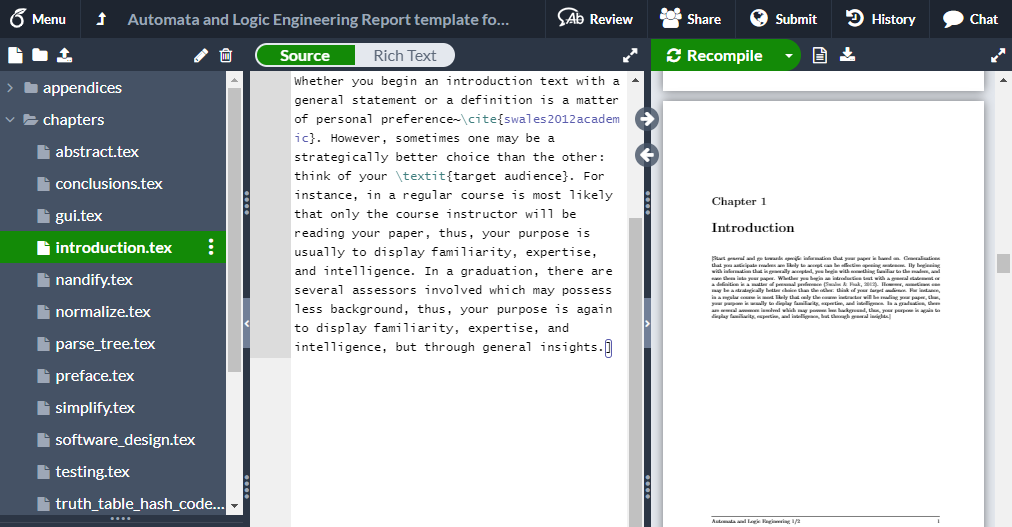
\includegraphics[width = \textwidth]{appendices/latex/latex_images/latex_example2.PNG}
    \caption{An example of LaTeX environment}
    \label{fig:latex_example}
\end{figure}

